\problemname{Gridvolleyboll}
Gridvolleyboll spelas med två spelare i varje lag (som beachvolley) men spelarna kan bara slå på bollen när de står på någon av de förutbestämda gridpunkterna.
Ett slag går till så att en spelare som står på en ``tillräckligt närliggande'' gridpunkt flyttar sig till den gridpunkt där bollen befinner sig.
Endast den spelare som just ska slå bollen får röra sig.
Spelaren bestämmer en gridpunkt dit hen vill slå bollen, antingen på den egna planhalvan (en ``passning'') eller på motståndarlagets planhalva (ett ``överslag'').
Bollen hamnar alltid på just den tilltänkta gridpunkten och kan inte snappas upp på vägen. 
Om det inte finns någon spelare som kan ta sig till gridpunkten där bollen är, så förlorar det lag där bollen befinner sig denna poäng.
Liksom i beachvolley får bollen slås högst tre gånger på en planhalva (två passningar och ett överslag), och samma person får inte slå bollen två gånger i rad.
Det första slaget (serven) ska alltid ske från ett av planens hörn och måste alltid vara ett direkt överslag.
Det är dessutom förutbestämt att den första spelaren ($A1$) i lag $A$ ska serva.

Skriv ett program som, givet planens storlek och de fyra spelarnas egenskaper, beräknar vilket lag som vinner poängen om båda lagen spelar optimalt.
Om inget av lagen kan tvinga sig till en vinst kommer bollen att pågå oändligt länge och vi räknar resultatet som oavgjort. 

Nätet är genomskinligt, så spelarna kan se motståndarlagets placering (men kom ihåg att man inte får röra sig förrän man ska slå bollen).
Spelet börjar på följande sätt: Först intar lag $A$ sina platser: spelare $A1$ i ett hörn och spelare $A2$ på valfri plats.
Därefter intar spelarna $B1$ och $B2$ sina (helt valfria) platser, medan lag $A$ inte får flytta sig.
Slutligen servar spelare $A1$ och spelet är igång.
Du kan anta att spelarna rör sig oberoende av varandra, de kan t.o.m. befinna sig på samma gridpunkt.
Däremot får de inte gå utanför planen eller in på motståndarnas planhalva.

\begin{figure}[h]
    \centering
    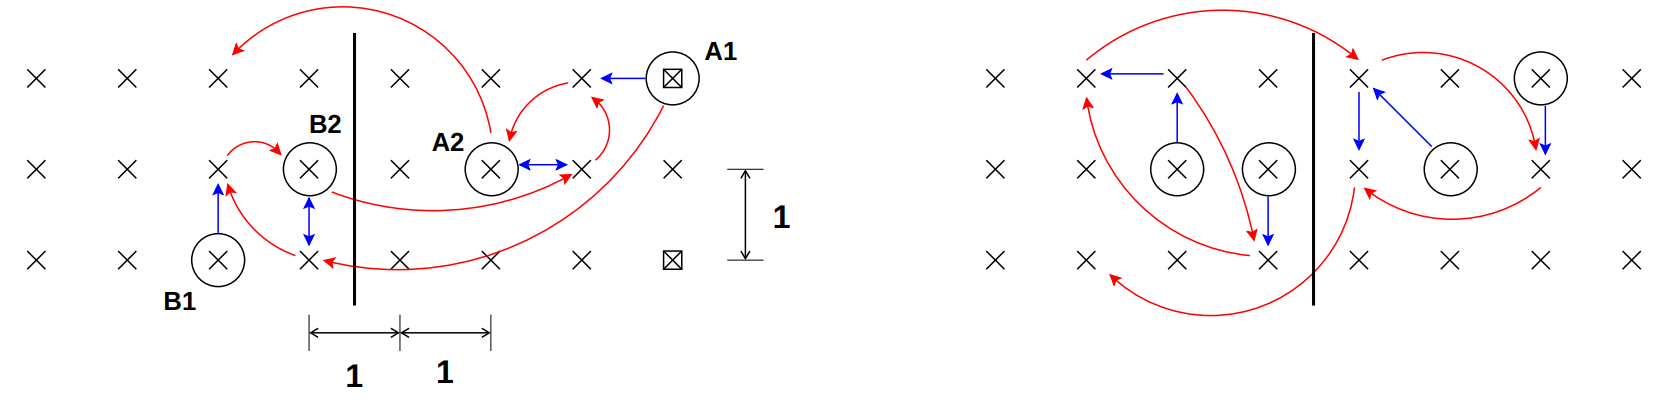
\includegraphics[width=1.0\textwidth]{grid}
    \caption{En möjlig spelsekvens i exempel $4$, där båda lagen spelar optimalt, d.v.s. lag $A$ spelar på ett sådant sätt att de garanterat vinner på högst $5$ överslag medan lag $B$ spelar på ett sådant sätt att lag $A$ inte kan vinna på mindre än $5$ överslag.
    Däremot finns det för båda lagen massor av likvärdiga spelsätt.
    Till vänster visas planens utformning med gridpunkterna markerade som kryss och de två möjliga servepunkterna markerade med kvadrater runt kryssen.
    Dessutom visas en utgångsställning för de fyra spelarna som är vinnande för lag $A$ och optimal för lag $B$.
    Vidare visas bollens väg med böjda röda pilar, medan spelarnas rörelser visas med blåa raka pilar.
    För tydlighets skull har spelsekvensen delats upp så att den vänstra figuren visar sekvensen till och med det tredje överslaget, och den högra figuren visar resten av sekvensen, som slutar med att lag $A$ slår över en boll som lag $B$ omöjligt kan ta.
    }
\end{figure}

\section*{Indata}
Den första raden innehåller talen $x$ ($2 \le X \le 4$) och $y$ ($2 \le Y \le 3$), antalet gridpunkter i $x$-led och $y$-led på varje planhalva (se figuren ovan).

Därefter följer fyra rader som vardera beskriver en spelare, i ordningen $A1$, $A2$, $B1$ och $B2$.
Varje rad består av två heltal $F$ ($0 \le F \le 25$)  och $S$ ($0 \le S \le 5$), där $\sqrt{F}$ är det maximala avståndet spelaren kan slå bollen och $\sqrt{S}$ är det maximala avståndet spelaren kan röra sig under ett slag, d.v.s. det maximala avståndet spelaren kan befinna sig från den gridpunkt dit bollen är på väg för att kunna nå den i tid.

\section*{Utdata}
Skriv först ut resultatet för lag $A$: \texttt{win}, \texttt{loss} eller \texttt{tie} för vinst, förlust eller oavgjort.
Om lag $A$ vinner ska programmet därefter skriva ut det minsta antalet överslag (båda lagens räknade) som krävs för att lag $A$ garanterat ska vinna (alltid udda antal).
Om lag $A$ förlorar ska programmet istället skriva ut det minsta antalet överslag (båda lagens räknade) som krävs för att lag $B$ garanterat ska vinna (alltid jämnt antal).
Om det blir oavgjort behöver inget tal skrivas ut.

\section*{Poängsättning}
Din lösning kommer att testas på en mängd testfallsgrupper.
För att få poäng för en grupp så måste du klara alla testfall i gruppen.

\textbf{Notera:} om ditt program endast beräknar resultatet korrekt men skriver ut fel minsta antalet överslag får du $30$ poäng på testgruppen.

\noindent
\begin{tabular}{| l | l | p{12cm} |}
  \hline
  Grupp & Poängvärde & Gränser \\ \hline
  $1$    & $50$        & Något lag kan alltid garanterat vinna.\\ \hline 
  $2$    & $50$        & Inga ytterligare gränser. \\ \hline 
\end{tabular}

